\section{Trabajo y Energía}

Hasta ahora hemos trabajado situaciones problemáticas con fuerzas constantes.
Si quisiéramos trabajar con fuerzas variables,
usar las leyes de Newton sería muy difícil.
Por ello,
el presente capítulo propone dos conceptos para trabajar este tipo de problemas:
\textbf{trabajo} y \textbf{energía}.

Además, será fundamental el \textbf{principio de conservación de la energía},
que sostiene que la energía es una cantidad se puede transformar,
pero no se puede crear ni destruir.

\subsection{Modelo sistema}

Hasta el capítulo anterior,
el principal modelo utilizado fue el modelo partícula.
En adelante, pondremos el foco en el modelo sistema.

Un sistema refiere a una porción del Universo,
que puede ser un objeto, una colección de objetos,
o una región del espacio.
Lo fundamental del concepto de sistema es considerar que tiene límites,
que delimitan una frontera con lo que denominamos \textbf{entorno}.

El modelo implica que hay \textit{mecanismos},
que sigue \textit{reglas},
mediante los cuales el sistema se relaciona con el entorno.
Por ejemplo,
si decimos que un objeto conforma nuestro sistema,
incorporando trabajo sobre él lo estaremos cargando de energía.

\subsection{Trabajo}

El trabajo, en mecánica,
se puede definir como el \textit{producto} entre
el \textbf{desplazamiento} de un objeto y el
\textbf{componente} de la fuerza \textit{paralelo} a ese desplazamiento.

\begin{equation*}
    W = \vec{F} \cdot \vec{d} \cdot \cos\theta
\end{equation*}

Donde \(\vec{F}\) es el vector fuerza,
\(\vec{d}\) es el vector desplazamiento
y \(\theta\) el ángulo entre ambos.

Notar que no es otra cosa que una de las expresiones para el producto punto
entre dos vectores.
Como es producto punto devuelve,
naturalmente, un \textit{escalar},
que no tiene dirección y puede ser negativo, positivo o cero.
Es negativo si los vectores son opuestos
(o la fuerza tiene componente opuesto)
y cero si la fuerza tiene dirección perpendicular al desplazamiento.

\vspace{.5cm}
\begin{center}
    Componente de \(\vec{F}\) paralelo y en mismo sentido de \(\vec{d}\): trabajo positivo
    \vspace{.25cm}

    \begin{tikzpicture}[>=stealth, scale=1]
        % ángulo
        \coordinate (A) at (1,0);
        \coordinate (B) at (0,0);
        \coordinate (C) at (33.69:1cm);

        \draw pic [draw=cyan!50!black, fill=cyan!20, angle radius=12mm,
                "$\theta$"] {angle = A--B--C};

        % nodo origen
        \fill (0,0) circle (2pt);

        % vector fuerza
        \draw[->, black, thick] (0,0) -- (3,2) node[above right] {$\vec{F}$};

        % vector desplazamiento
        \draw[->, blue, thick] (0,0) -- (5,0) node[above right] {$\vec{d}$};

        % Componente fuerza paralelo al desplazamiento
        \draw[cyan, dashed] (3,2) -- (3,0);
        \draw[->, gray, thick] (0,0) -- (3,0) node[below right] {$(+)\,\vec{F_x}$};
    \end{tikzpicture}
\end{center}

\vspace{.5cm}
\begin{center}
    Componente de \(\vec{F}\) perpedicular a \(\vec{d}\): trabajo nulo
    \vspace{.25cm}

    \begin{tikzpicture}[>=stealth, scale=1]
        % ángulo
        \coordinate (A) at (1,0);
        \coordinate (B) at (0,0);
        \coordinate (C) at (90:1cm);

        \draw pic [draw=cyan!50!black, fill=cyan!20, angle radius=12mm,
                "$\theta$"] {angle = A--B--C};


        % nodo origen
        \fill (0,0) circle (2pt);

        % vector fuerza
        \draw[->, black, thick] (0,0) -- (0,3) node[above right] {$\vec{F}$};

        % vector desplazamiento
        \draw[->, blue, thick] (0,0) -- (5,0) node[above right] {$\vec{d}$};

        % Componente nulo
        \fill[gray] (0,0) circle (1.5pt) node[below left] {$(0)\,\vec{F_x}$};
    \end{tikzpicture}
\end{center}

\vspace{.5cm}
\begin{center}
    Componente de \(\vec{F}\) paralelo y en sentido contrario de \(\vec{d}\):
    trabajo negativo
    \vspace{.25cm}

    \begin{tikzpicture}[>=stealth, scale=1]
        % ángulo
        \coordinate (A) at (1,0);
        \coordinate (B) at (0,0);
        \coordinate (C) at (146.31:1cm);

        \draw pic [draw=cyan!50!black, fill=cyan!20, angle radius=12mm,
                "$\theta$"] {angle = A--B--C};


        % nodo origen
        \fill (0,0) circle (2pt);

        % vector fuerza
        \draw[->, black, thick] (0,0) -- (-3,2) node[above right] {$\vec{F}$};

        % vector desplazamiento
        \draw[->, blue, thick] (0,0) -- (5,0) node[above right] {$\vec{d}$};

        % Componente paralelo al desplazamiento
        \draw[cyan, dashed] (-3,2) -- (-3,0);
        \draw[->, gray, thick] (0,0) -- (-3,0) node[below right] {$(-)\,\vec{F_x}$};
    \end{tikzpicture}
\end{center}
\vspace{.5cm}

Para no errarle, usar la expresión del \textit{producto punto entre vectores}:

\begin{equation*}
    W = \vec{F} \cdot \vec{d} = |F| \cdot |d| \cdot \cos\theta
\end{equation*}

La unidad en que se mide el trabajo en el SI es el \textbf{joule} \((J)\).
El trabajo se mide como el producto de \textit{fuerza por distancia},
por lo tanto \(J = N \cdot m\).

En el sistema británico la unidad de trabajo es el \textit{pie-libra} \((ft \cdot lb)\).
La equivalencia es \(1 J = 0.7376 ft \cdot lb\).

El \textbf{trabajo total} se puede calcular sumando algebraicamente el trabajo 
de cada fuerza -teniendo en cuenta los signos-, o calculando el trabajo que 
realiza la \textit{fuerza neta}.

\subsection{Trabajo con fuerza cambiante}

Veremos que el teorema del trabajo y la energía se cumple para los casos más 
generales que implican \textbf{fuerza variable} y \textbf{trayectoria no rectilínea}.

Primero, veamos la fuerza variable.

La fuerza que hace un resorte es directamente proporcional al estiramiento
-o presión- más allá de su longitud natural\footnote{Siempre que el alargamiento no sea excesivo.}:

\begin{equation*}
    f = -kx
\end{equation*}

Donde \(f\) es la fuerza, \(k\) la constante elástica, medida en \(N/m\)
y \(x\) la longitud de estiramiento o compresión del resorte.
Esta expresión se conoce como \textbf{ley de Hooke}, por Robert Hooke que la 
observó en 1678.
Lleva signo negativo porque el sentido de la fuerza es contrario al sentido 
del estiramiento: si nos vamos a la derecha, la fuerza es hacia la izquierda.
Por el contrario, si presionamos hacia la izquierda la fuerza del resorte va 
paralela pero en sentido contrario.

Para conocer el trabajo en función de la distancia operamos integral sobre 
la ley de Hooke:

\begin{equation*}
    \int_{0}^{X} f \; dx = \int_{0}^{X} -kx \; dx = \frac{-kx^{2}}{2}
\end{equation*}

Es decir,
el trabajo realizado crece con el cuadrado de la distancia,
manteniendo así el teorema del trabajo y la energía.

\subsection{Trabajo y energía cinética}

El trabajo se relaciona con el desplazamiento de un objeto,
pero también con los \textbf{cambios en su rapidez}.

Dada una fuerza constante sobre un cuerpo,
que consecuentemente tendrá aceleración constante,
llegamos a la expresión:

\begin{equation*}
    W = \frac{1}{2}mV_f^{2} - \frac{1}{2}mV_i^{2} 
\end{equation*}

La expresión \(\frac{1}{2}mV^{2}\) se define como \textbf{energía cinética} \((K)\).
De manera tal que podemos expresar el 
\textit{teorema del trabajo y la energía cinética} como: 

\begin{equation*}
    W = \Delta K
\end{equation*}

Es decir,
cuando aplicamos trabajo sobre un sistema y su único cambio es en la rapidez,
podemos afirmar que el trabajo es igual a la energía cinética del sistema.
Una partícula gana energía cinética porque interactúá con otros objetos,
que ejercen fuerza sobre ella.

Ya hemos visto que el teorema del trabajo y la energía se cumple para una 
trayectoria recta. ¿Qué pasa con una trayectoria curva?

En primer lugar, si el cuerpo tuviera solo aceleración centrípeta,
pero no tuviera aceleración tangencial,
estamos ante un cuerpo que no tiene una fuerza en el sentido del desplazamiento.
Por lo tanto, el trabajo sería 0.

En una segunda situación, podemos plantear que el cuerpo tiene aceleración 
tangencial además de la centrípeta. Por lo tanto, hay una fuerza tangencial,
que sigue la expresión: \(F\cdot\cos\theta = F_x\).
Si operamos integral sobre ese componente:

\begin{equation*}
    \int_{x_1}^{x_2} F_x \; dx = F_x \cdot \vec{d}
\end{equation*}

Es decir, el teorema del trabajo y la energía se cumple también para una 
trayectoria no rectilínea.

Una última característica de la energía cinética:
una vez que el sistema recibe trabajo e incrementa su energía,
tiene a su vez la capacidad de realizar un trabajo.
¿Qué trabajo realiza la energía cinética?
Puede, por ejemplo, si colisiona con otro cuerpo, entregar su energía cinética,
poniendo en movimiento al segundo cuerpo:
la energía cinética es igual al trabajo efectuado para poner el cuerpo 
en movimiento,
y es igual también al trabajo que puede efectuar cuando se detiene.

\subsection{Energía potencial}

Si un cuerpo con energía cinética recorre un camino sinuoso:

\begin{figure}[H]
    \centering
    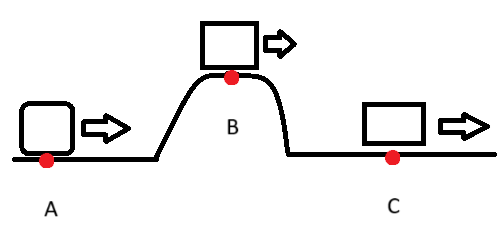
\includegraphics[width=.7\textwidth]{img/04-energia-potencial.png}
\end{figure}

En el punto \(A\) va a tener una energía cinética.
A medida que sube hacia \(B\), suponiendo que no hay fricción,
pierde igualmente velocidad.
En cuanto vuelve a bajar a \(C\), que está a la misma altura de \(A\),
recupera la velocidad. ¿Cómo se entiende este fenómeno?

Siguiendo el \textbf{principio de conservación de la energía}, 
la energía cinética se convierte en otro tipo de energía,
que llamamos \textbf{energía potencial} \((U)\).

La suma de la energía potencial y la energía cinética se denomina 
\textbf{energía mecánica} \((E_m = K + U)\),
que permanece constante para todo el desplazamiento,
cumpliendo así con el principio de conservación.

De esto se desprende una idea interesante:
hay energía asociada a la posición de los cuerpos en un sistema.
En este caso, el sistema conformado por el objeto y la Tierra,
que ejerce \textit{fuerza gravitacional} sobre el objeto en altura,
dándole la posibilidad de recuperar la velocidad.
Por eso hablamos de \textbf{energía potencial gravitacional}.
Aunque, normalmente, nos referiremos a la energía potencial del objeto,
en realidad corresponde al sistema objeto-Tierra. 
La energía potencial de un cuerpo aislado no tendría sentido.

Si asignamos un valor nulo a la energía potencial gravitatoria sobre la 
superficie terrestre, \(U = 0\), a medida que el cuerpo se eleva de la 
superficie adquiere energía potencial siguiendo la expresión:

\begin{equation*}
    U = mgh
\end{equation*}

Siendo \(m\) la masa del objeto, \(g\) la aceleración debida a la fuerza 
gravitatoria terrestre y \(h\) la altura.

Sin embargo, esta no es la única energía potencial.
Un cuerpo deformable elástico,
esto es, un cuerpo que puede deformarse pero que recupera su forma y tamaño 
original cuando se suelta,
como un resorte,
almacena \textbf{energía potencial elástica},
que sigue la expresión:

\begin{equation*}
    U_{el} = \frac{1}{2}kx^{2}
\end{equation*}

Siendo \(k\) 